\documentclass{article}
\usepackage{amsmath}
\usepackage{mathtools}
\usepackage{gensymb}
\usepackage[a4paper,inner=1.5cm,outer=1.5cm,top=2cm,bottom=0.5cm]{geometry} 
\usepackage{xcolor}                    
\usepackage{tikz}                           
\usepackage{multicol}
\usepackage{pgfplots}
\usetikzlibrary{calc}
\usetikzlibrary{intersections}
\usetikzlibrary{intersections,calc,angles,quotes}
\usetikzlibrary{shapes,arrows,positioning,decorations.pathreplacing,calc}
\usetikzlibrary{calc,angles,positioning,intersections,quotes,decorations.markings}
\usepackage{tkz-euclide}
\usetikzlibrary{backgrounds}
\usetikzlibrary{calc,through}
\usetikzlibrary{angles}
\usetikzlibrary{fadings}
\usetikzlibrary{shapes.geometric}
\usetikzlibrary{shapes.symbols}
\usepackage{draftwatermark}
\usepackage{mathptmx}

\SetWatermarkText{\textcolor{black!20}{Mathema Shukur}}
\SetWatermarkFontSize{2 cm}
\usepackage[utf8]{inputenc}
\usepackage{fontspec}

\setmainfont{[Kalpurush.ttf]}
\newfontface{\en}{[Arial.ttf]} %%this is optional, if you want to use a secondary font. Any english font is supported
\newlength\Radius
\setlength\Radius{4cm}
\begin{document} 
	\Large
	\textcolor{red}{Welcome To} 
	\\
	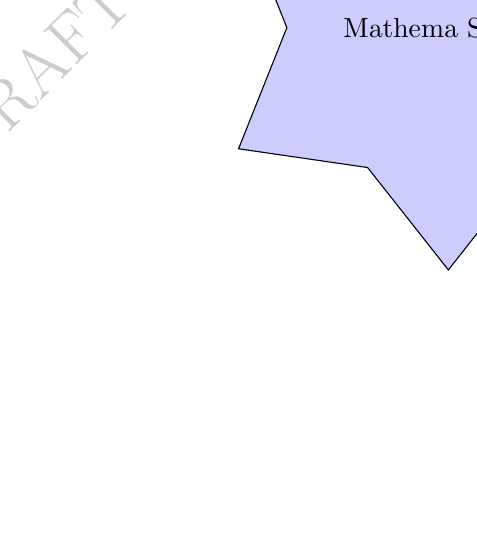
\begin{tikzpicture}
		\tikz \node [fill=blue!20,star,star points=6,draw] {Mathema Shukur };
	\end{tikzpicture}
	\\
	যাদের জন্যে প্রযোজ্যঃ  	\textcolor{magenta}{একাদশ ও দ্বাদশ শ্রেণীর শিক্ষার্থী} \\
	বিষয়ঃ \textcolor{magenta}{উচ্চতর গণিত ১ম পত্র} \\
	অধ্যায়ঃ \textcolor{magenta}{৪-বৃত্ত}\\ 
	\\
	\\
	(১)  মূল বিন্দুতে কেন্দ্র বিশিষ্ট বৃত্তের সমীকরণ  \\
	\\
	\textcolor{blue}{$x^2+y^2=r^2$}\\
	\\
	(২) নির্দিষ্ট কেন্দ্র ও ব্যাসার্ধ বিশিষ্ট বৃত্তের  সমীকরণ \\
	\\
	\textcolor{blue}{$(x-h)^2+(y-k)^2=r^2$}\\
	\\
	(৩) বৃত্তের সাধারণ সমীকরণ\\
	\\  
	\textcolor{blue}{$x^2+y^2+2gx+2fy+c=0$}\\
	\\
	(৪) ব্যাসের প্রান্ত বিন্দুদ্বয় $(x_1,y_1)$ এবং $(x_2,y_2)$ হলে বৃত্তের সমীকরণ\\
	\\ 
	\textcolor{blue}{$(x-x_1)(x-x_2)+(y-y_1)(y-y_2)=0$}\\
	\\
	(৫) একটি বৃত্ত \textcolor{blue}{$S=0$ }এবং একটি সরলরেখা \textcolor{blue}{$L=0$}  এর ছেদবিন্দুগামী বৃত্তের সমীকরণ  \textcolor{blue}{$S+kL=0$} \\
	\\
	(৬) দুইটি বৃত্ত \textcolor{blue}{$S_1=0$} ও \textcolor{blue}{$S_2=0$} এর ছেদবিন্দুগামী বৃত্তের সমীকরণ \textcolor{blue}{$S_1+kS_2=0$}\\  \\
	(৭) পোলার স্থানাঙ্কে বৃত্তের  সমীকরণ \\
	\textcolor{blue}{$r^2+2r(g\cos \theta+f\sin \theta )+c=0$}\\
	যেখানে 	$g=-\rho \cos \alpha,\,\,\,f=-\rho \sin \alpha,\,\,\,c=\rho^2-a^2 $\\
	\\ 
		\textcolor{blue}{[ঢাকা বোর্ড-২০১১]}\\
একটি বৃত্তের সমীকরণ নির্ণয় কর যা মূলবিন্দু এবং $\textcolor{blue}{x^2+y^2-2x-4y-4=0}$ বৃত্ত  ও  $\textcolor{blue}{2x+3y+1=0}$ রেখার ছেদ বিন্দু দিয়ে যায়। 
	\begin{tikzpicture}[transform shape,scale=1]
	\draw [-latex,thick,red](-7,0) -- (4,0) node[right] {$x$} coordinate(x axis);
	\draw [-latex,thick,red](0,-9) -- (0,6) node[above] {$y$} coordinate(y axis);
	\fill[black] (0,0) circle (1 mm);
	\node at (0.8,-0.3) {$\textcolor{red}{O(0,0)}$};	
	\draw[thick,blue] (1,2) circle (3);
	\draw[blue](-5,3)--(4,-3);
	\draw[thick,green,dashed] (-3,-4) circle (5);
\end{tikzpicture}\\
	\begin{align*}
	S+kL&=0\\
	\\ 
	(x^2+y^2-2x-4y-4)+k(2x+3y+1)&=0\\
	\\
	x^2+y^2-2x-4y-4+2kx+3ky+k&=0\\
	\\
	x^2+y^2+(2k-2)x+(3k-4)y+k-4&=0\hspace{1cm}[EQ01]\\
	\boxed{\textcolor{blue}{x=0,\,\,y=0}}&\\
	(0)^2+(0)^2+(2k-2)(0)+(3k-4)(0)+k-4&=0\\
	\\
	k&=4
\end{align*}
\begin{align*}
	x^2+y^2+(2k-2)x+(3k-4)y+k-4&=0\hspace{1cm}[EQ01]\\
	\boxed{\textcolor{blue}{k=4}}&\\
	x^2+y^2+(8-2)x+(12-4)y+4-4&=0\\
	\\
	x^2+y^2+6x+8y&=0\\	
\end{align*}


		\textcolor{blue}{[দিনাজপুর  বোর্ড-২০১৪]}\\
	একটি বৃত্তের সমীকরণ নির্ণয় কর যার কেন্দ্র $(6,0)$ এবং যা $\textcolor{blue}{x^2+y^2-4x=0}$ বৃত্ত ও  $\textcolor{blue}{x=3}$ রেখার ছেদ বিন্দু দিয়ে যায়। 
	\\
	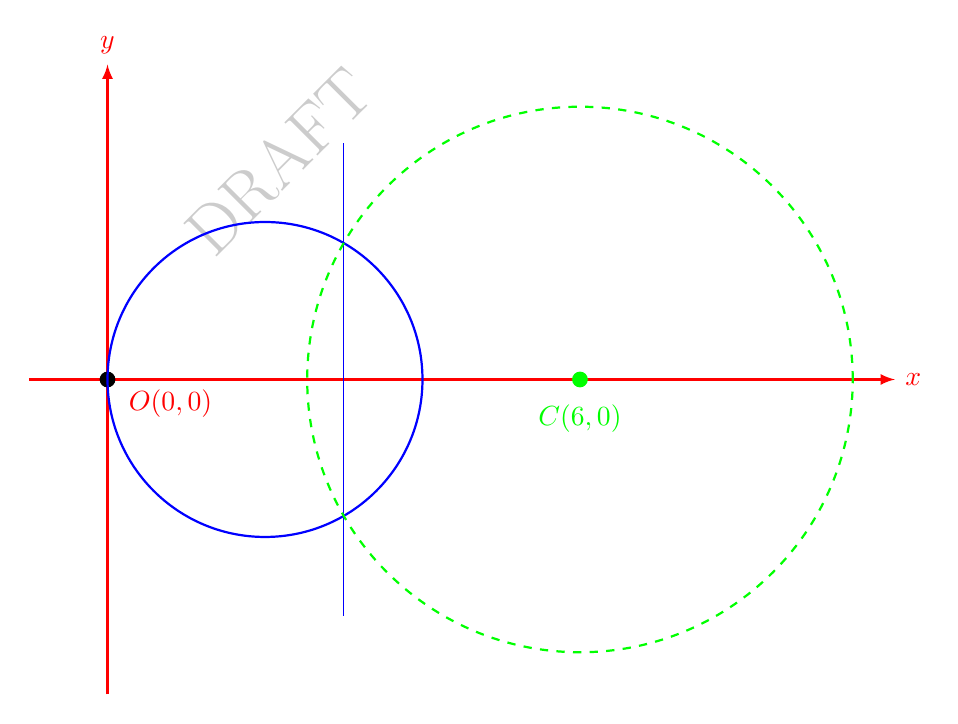
\begin{tikzpicture}[transform shape,scale=1]
		\draw [-latex,thick,red](-1,0) -- (10,0) node[right] {$x$} coordinate(x axis);
		\draw [-latex,thick,red](0,-4) -- (0,4) node[above] {$y$} coordinate(y axis);
		\fill[black] (0,0) circle (1 mm);
		\node at (0.8,-0.3) {$\textcolor{red}{O(0,0)}$};	
		\draw[thick,blue] (2,0) circle (2);
		\node at (6,-0.5) {$\textcolor{green}{C(6,0)}$};
		\fill[green] (6,0) circle (1 mm);
		\draw[blue](3,3)--(3,-3);
		\draw[thick,green,dashed] (6,0) circle (3.464);
	\end{tikzpicture}\\
	\\
	\begin{align*}
		S+kL&=0\\
		\\ 
	(x^2+y^2-4x)+k(x-3)&=0\\
	\\
	x^2+y^2-4x+kx-3k&=0\\
	\\
	x^2+y^2+(k-4)x-3k&=0\hspace{1cm}[EQ01]\\
	\boxed{\textcolor{blue}{x^2+y^2+2gx+2fy+c=0}}&\\
	x^2+y^2+2\left(\frac{k-4}{2}\right)x+2(0)y+(-3k)&=0\\
\\
	g=\left(\frac{k-4}{2}\right);\,\,\,f=&0;\,\,\,c=-3k
	\end{align*}
কেন্দ্র $(-g,-f)=\left(-\frac{k-4}{2},0\right)=(6,0)$\\
\\
$-\frac{k-4}{2}=6$\\ 
$k-4=-12$\\
$k=-8$\\
	\begin{align*}
	x^2+y^2+(k-4)x-3k&=0\hspace{1cm}[EQ01]\\
	\\
		\boxed{\textcolor{blue}{k=-8}}&\\
	\\
		x^2+y^2+(-8-4)x-3(-8)&=0\\
		\\
		x^2+y^2-12x+24&=0
\end{align*}
\end{document}